\documentclass[11pt]{aghdpl}
% \documentclass[en,11pt]{aghdpl}  % praca w języku angielskim
\usepackage[polish]{babel}
%\usepackage[english]{babel}
\usepackage[utf8]{inputenc}

% dodatkowe pakiety
\usepackage{enumerate}
\usepackage{listings}
\lstloadlanguages{TeX}

\lstset{
  literate={ą}{{\k{a}}}1
           {ć}{{\'c}}1
           {ę}{{\k{e}}}1
           {ó}{{\'o}}1
           {ń}{{\'n}}1
           {ł}{{\l{}}}1
           {ś}{{\'s}}1
           {ź}{{\'z}}1
           {ż}{{\.z}}1
           {Ą}{{\k{A}}}1
           {Ć}{{\'C}}1
           {Ę}{{\k{E}}}1
           {Ó}{{\'O}}1
           {Ń}{{\'N}}1
           {Ł}{{\L{}}}1
           {Ś}{{\'S}}1
           {Ź}{{\'Z}}1
           {Ż}{{\.Z}}1
}

%---------------------------------------------------------------------------

\author{Krzysztof Romanowski}
\shortauthor{K. Romanowski}

\titlePL{Debuggowanie aplikacji kominukujących się asynchronicznie oparte o historię komunikatów.}
\titleEN{History-based approach for debugging applications using asynchronous communication.}

\shorttitlePL{Debugowanie} % skrócona wersja tytułu jeśli jest bardzo długi
\shorttitleEN{Debugging}

\thesistype{Praca dyplomowa magisterska}
%\thesistype{Master of Science Thesis}

\supervisor{dr hab. Arkadiusz Janik, dr inż}
%\supervisor{Marcin Szpyrka PhD, DSc}

\degreeprogramme{Informatyka}
%\degreeprogramme{Computer Science}

\date{2015}

\department{Katedra Informatyki}

\faculty{Wydział Elektrotechniki, Automatyki, Elektroniki i Telekomunikacji}

\acknowledgements{Serdecznie dziękuję \dots tu ciąg dalszych podziękowań np. dla promotora, żony, sąsiada itp.}


\setlength{\cftsecnumwidth}{10mm}

%---------------------------------------------------------------------------
\setcounter{secnumdepth}{4}

\begin{document}

\titlepages
\setcounter{tocdepth}{3}
\tableofcontents
\clearpage

\chapter{Wprowadzenie}

%---------------------------------------------------------------------------

\section{Motywacja}

Podczas tworzenia aplikacji asychronicznych twórcy wielokrotnie napotykają ograniczenia narzędzi, które nie są przystosowane do pracy z tą klasą aplikacji. Podstawowe techniki, takie jak analiza wyjątków czy klasyczne debuggery, przeważnie nie dają wystarczających informacji o naturze problemów. Iulian Dragos w swojej prezentacji \cite{rethingningDebugger} przedstawił koncepję asychronicznego debuggera, przeznaczonego do debugowania aplikacji stworzonych przy wykorzystaniu technologii Akka oraz mechanizmu Feature'ów z języka Scala. Po wysłuchaniu prelekcji uznałem, że przedstawiona przez Dragos'a koncepcja jest dobra, jednakże wykorzystane tutaj sposoby persystencji komunikatów będą miały zbyt duży wpływ na działania debuggowanej aplikacji.



\section{Cele pracy}


Celem poniższej pracy jest zbadanie możliwości oraz efektywaności debugowania aplikacji komunikujących się asynchronicznie w oparciu o historię komunikatów. Głównym obszarem zainteresowań pracy będą pomiar oraz zmieniejszenie narzutu sposobu persystowania i analizy komunikatów na czas wykonywania poszczególnych części aplikacji. Zamierzam zaimplementować i przetestować różne podejścia, a następnie zestawić wyniki z ograniczeniami danej metody. Ponieważ jednak przedmiotem tej pracy nie jest stworzenie asynchronicznego debuggera, wykorzystam pracę Iuliana \cite{asychDebuggerGh}. Zaimpelementowany debugger jest częścią ScalaIDE – IDE dedykowanego Scali. Przetestuję wydajność, wykorzystując aplikacje napisane w frameworku Akka – najpopularniejszej technologii do pisania aplikacji asychronicznych, opartych o wymianę komunikatów w ekosystemie Scali.














\chapter{Asychroniczny debugger}

W tym rozdziale zamierzam przedstawić zasadę działania wykorzystanego asynchronicznego debuggera na tle narzędzi oferowanych przez JVM. Zamierzam nakreślić problemy oraz sposoby ich rozwiązywania oraz pokazać dlaczego sposób perysytencji komunikatów jest kluczowy dla minimalizacji wpływu debuggera na debugowaną aplikacje. 

%---------------------------------------------------------------------------

\section{Techniki i narzędzia służących do debuggowania}

W tym podrozdziale przedstawię techniki oraz narzędzia służące analizie i debugowaniu aplikacji które udostępnia ekosystem JVM. Zamierzam również pokazać dlaczego narzędzia te są niewystrczające do debugowania programów asychronicznych.

\subsection{Wyjątki i ich analiza}
Duża część błędów w programie kończy się rzuceniem wyjątku. Poza informacją o rodzaju wyjątku oraz komunikatem błędu JVM udostępnia nam stack trace.

\begin{quote}
A Stack Trace is a list of method calls from the point when the application was started to the point where the exception was thrown. The most recent method calls are at the top.~\cite{javaProgramming}
\end{quote} 

Stack trace jest niezwykle przydatny przy śledzeniu wywołania gdyż błędy często biorą się ze złego kontekstu wywołania metody (np. wykorzystanie niewłaściwej metody czy nieskończona rekurusja). Dzięki jego analizie jesteśmy w stanie odtworzyć historie wywołań oraz znaleźć kontekst w którym wyjątek został rzucony. Co więcej analiza stack trace'ów pozwala nam na odtworzenie w pewnych sytuacjach parametrów metody czy wartości pól w obiektach.
Niestety stack trace udostępnia nam tylko stos wywołań metod w pojedynczym wątku. Logika (potok logiki) w aplikacjach asychronicznych jest przeważnie rozrzucony po wielu wątkach. Przykładowy stack trace z applikacji w fameworku Akka:

\begin{quote}
TODO wyjątek
\end{quote}

Załączony listing daje nam informacje o stosie wywołań od odebrania ostatniej wiadomości. W przeważającej liczbie przypadków są to informacje niewystarczające gdyż przeważnie nie pozawala nam to na odtworzenie cyklu wiadomości które doprowadziły do powstania wyjątku.

\subsection{Tracing}

Jest to dość proste i naiwne podejście do debugowania polegające logowaniu punktów w aplikacji (na standardowe wyjście lub w inne miejsce, np. do pliku) i późniejszej analizie (przeważnie post mortem). Podstawową wadą tego rozwiązania jest konieczność ponownej kompilacji kodu dla każdej fali dodawania kolejnych logów. Po poprawieniu błędów programiści często zapominają o usunięciu wszystkich logowanych komunikatów co zaśmieca logi czy kod źródłowy a nawet potrafi być przyczyną problemów.
Rozwiązanie mimo swojej prosty ma szereg zalet. Nie wymaga żadnych specjalistycznych narzędzi ani umiejętności. Posiada także całkiem mały wpływ na wykonanie aplikacji lecz w przypadku aplikacji wielowątkowych wymaga zastosowania bardziej zaawansowanych technik (takich jak dedykowany plik dla każdego wątku). 
Mimo swej prostoty rozwiązanie to jest szeroko stosowane przez programistów. W przypadku aplikacji asychronicznych często jest jednym dostępnym sposobem debugowania. 

\subsection{Instrumentacja kodu}

TODO Pisać o tym???
Instrumentacja kodu jest przeważnie wykorzystywana do zautomatyowanego tracingu.

\subsection{Debugger}
Debugger jest programem do dynamicznej analizy wykonania innych programów. 
\begin{quote}
    With the magic of including debugging symbols in the executable, the debugger gives the illusion of executing the program line by line of source code, instead of instruction by instruction of compiled machine code~\cite{artOfDebugging}
\end{quote}
Odwzorowanie kodu maszynowego na kod źródłowy jest skomplikowanym zadaniem, zwłaszcza dla języków wysokopoziomowych. Współczesne debuggery opierają swoje działanie o mechanizm breakpointów czyli definicji miejsc w których wykonanie programu powinno zostać wstrzymane (czasem tylko w celu zalogowania komunikatu - debugger może być także wykorzystany do tracing'u). Po wstrzymaniu działania użytkownik może przeglądać wartości zmiennych, pól czy w bardziej zaawansowanych debuggerach ewaluować wyrażenia.
Debugger pozwala także na sterowanie wykonaniem programu. Poza komendami które nie ingerują w normalne wykonanie programu (Step in, Step out, Step into itp.) pozwala także na np. pownowe wykonanie funkcji (drop frame).

Niestety debuggery dostępne dla aplikacji działających na JVM mają te samą wadę co analiza wyjątków. Są skuteczne tylko do analizy logiki w ramach pojedynczego wątku. Jest to spowodowane architekturą JVM oraz udostępnianymi przez nią narzędziami.

% Dalsza część jest mocno pogądowa i nie nadaje się za bardzo do czytania (poza tytułami rozdziałów

\section{debugowanie na JVM}

W tym podrozdziale zamierzam przedstawić JVM w kontekście debugowania aplikacji asynchronicznych. Zmierzam pokazać że potok wywoływania kodu maszynowego różni się koncepcyjnie od potoku przetwarzania komunikatów przez aplikację asynchroniczne. Zamierzam także przestawić właściwości Java Platform Debugger Architecture na których opiera się działania Asychronicznego Debuggera.

\subsection{JVM: wątki}

TODO - opisać stosowość i przypisanie do wątku. Pokazać dlaczego rozdzięk między logiką opartą na komunikatach a na wywołaniach metody

\subsection{Architektura JDPA}

Jako że każdy debugger jest odzielną aplikacją, Java Platform Debugger Architecture składa się z trzech koponentów przedstawionych na wykresie:

\includegraphics{imgs/jdpa}

1. JVM TI: instrumentacja JVM

Java™ Virtual Machine Tool Interface służy instrumentacji debuggej JVM.

\begin{quote}
The JVMTM Tool Interface (JVM TI) is a programming interface used by development and monitoring tools. It provides both a way to inspect the state and to control the execution of applications running in the JavaTM virtual machine (VM). \cite{jvmtiSpec}
\end{quote}

Nie jest to tylko narzędzie do debugowania ale może być także podstawą dla tworzenia innych narzedzi takich jak np. profilery.

Aspektem który nas najbardziej interesuje jest niskopoziomowa obsługa breakpointów. Mechanizm działania jest podzielony na 2 etapy:

1. Deklaracja breakpointu
2. Obsługa eventu wygenerowanego przez breakpoint (tu następuje decyzja czy zatrzymać wykonywanie czy nie)

JVM TI pozwala nam także na dostęp do zmiennych lokalnych oraz parametrów metod. Pozwoli nam to na przechwytywanie przesłanych komunikatów bez udziału debbugera a co za tym idzie przyspieszenie całego procesu, gdyż komunikacja między dwiema aplikacjami jest kosztowna.


2. JDWP: protokół transportowy

Java Debug Wire Protocol: protokół transportowy wykożystywany do komunikacji między maszyną wirtualną (JVM TI) a debuggerem (lub innym programem takim jak profiler). W asychronicznym debuggerze korzystamy z imlementacji dostarczanej przez JDT. W wiekszości przypadków komunikacja jest schowana za warstwą abstracji implementują JDI. Więcej informacji możemy znaleść w specyfikacji\cite{jwdpSpec}

3. JDI: wysokopoziomowe API

Wysokopoziomowe API służace do tworzenia debuggerów i innych narzędzi programistycych (np. profilerów). Podobnie jak JDWP jest zaimplementowany przez JDT i stanowi wysokopoziomowe API które jest podstawą debuggera.
Zawiera metody pozwalające na:
- deklarowanie breakpointów
- obsługę eventów (np. zatrzymanie na breakpoint'cie)
- dostęp do obiektów (parametrów metod, zmiennych lokalnych czy statycnych pól),
- wywoływanie metod i tworzenie nowych instacji
- sterowanie wywołaniem aplikacji

Większość wymienionych metod zostanie wykorzystana do stworzenia asychronicznego debugera.

\subsection{Narzędia udostępniane przez JDPA}

TODO: opisać breakpoint, code evaluation itp. - to co bedziemy wykorzystywać.

\section{Zasada dzialania}

W tym podrozdziale zamierzam przedstawić zasadedziałania asychronicznego debuggera oraz nakreślić  miejsca które będą przedmiotem tej pracy.

\subsection{Asychrnoniczna historia wywołań}
TODO
\subsection{Historia komunikatów}
TODO
\subsection{Budowanie historii komunikatów}

TODO

\subsection{Asychroniczne debuggowanie aplikacji aktorowych: Akka}
\chapter{Rozdział do testów}

Brak sensownej zawartości ;)



\chapter{Sposoby tworzenie historii komunikatów}

W tym rozdiale zamierzem przedstawić sposoby tworzenia historii komunikatów. Zamierzam podzielić ten proces na dwa etapy i przedstawić sposoby ich implementacji. W ostatnim podrozdiale zamierzam przedstawić testowane sposoby (złożenia). 

\section{Dwa etapy: zbieranie i wysyłanie danych}

\section{Metody zbierania danych}

\subsection{Plain JDI}

\subsection{JVM TI: Java Agent}

\subsection{JDI: instrumentacja kodu}

\section{Metody przesyłania danych}

\subsection{Plain JDI}

\subsection{Plain JDI: lazy mode}

\subsection{Filesystem}

\subsection{Socets}

\section{Testowane złożenia}

TODO: wyjdzie podczas implementacji
\chapter{Wyniki oraz ich a analiza}

\section{Aplickacja 1}
\subsection{Test 1}
\subsection{Test 2}
\subsection{Test 3}
\subsection{Analiza}

\section{Aplickacja 2}
\subsection{Test 1}
\subsection{Test 2}
\subsection{Test 3}
\subsection{Analiza}

\section{Zestawienie zbiorcze}
\subsection{Test 1}
\subsection{Test 2}
\subsection{Test 3}
\subsection{Analiza}
\chapter{Analiza oraz wnioski}

TODO: w zależności co wyjdzie

\section{Dalsze możlowości rozwoju}




% itd.
% \appendix
% \include{dodatekA}
% \includegraphics[scale=•]{•}{dodatekB}
% itd.
\bibliographystyle{alpha}
\bibliography{bibliografia}


\end{document}
